%%% Thesis Introduction --------------------------------------------------
\chapter{Introduction}
\ifpdf
    \graphicspath{{Introduction/IntroductionFigs/PNG/}{Introduction/IntroductionFigs/PDF/}{Introduction/IntroductionFigs/}}
\else
    \graphicspath{{Introduction/IntroductionFigs/EPS/}{Introduction/IntroductionFigs/}}
\fi

Synergy organization started its work in a group since 2004 in Indore Madhya Pradesh and was registered on May 15, 2006. The early members who were mainly youngsters started working among the slums of Indore city. Later on it was felt by the youth to form such group, which can perform better in the fields of social services giving special focus to awareness in the slum area like AIDS, hygiene, immunization and education. Thus the name ``SYNERGY'' was carved out of the experience from the works through participatory action and energetic. \newline

\begin{figure}[!htbp]
  \begin{center}
    \leavevmode
    \ifpdf
      
\includegraphics[height=2in]{logo}
    \else
      
\includegraphics[bb = 92 86 545 742, height=6in]{logo}
    \fi
    \caption{Synergy Sansthan Logo}
    \label{FigAir}
  \end{center}
\end{figure}


Synergy is the group of some devoted youth who are committed to serve the poverty stricken and vulnerable people with special attention to empower women, children and local self-governance. In the fast changing socio-economic condition, social security becomes an issue of major concern. With rapid deterioration in moral, traditional and cultural values, changing climatic conditions due to environmental degradation and frequent natural disasters, the reality is changing rapidly. The rise in crime rate, number of orphanages, old age homes etc. are the result of waning human empathy. So in this situation Synergy believes in creating a society that is sustainable and is free from exploitation of humans and natural resources and by proving equal opportunity to the marginalized, poor, women and children to develop. It also makes efforts in making a society with sustainable human development and building capacity, sharing common vision of institution and nation building and reinforcing human development endeavors for over all progress of mankind. Synergy also believes in participatory action at the community level.
%%% ----------------------------------------------------------------------

\begin{figure}[ht!]
	\begin{subfigure}{.5\textwidth}
	  	\centering
	  	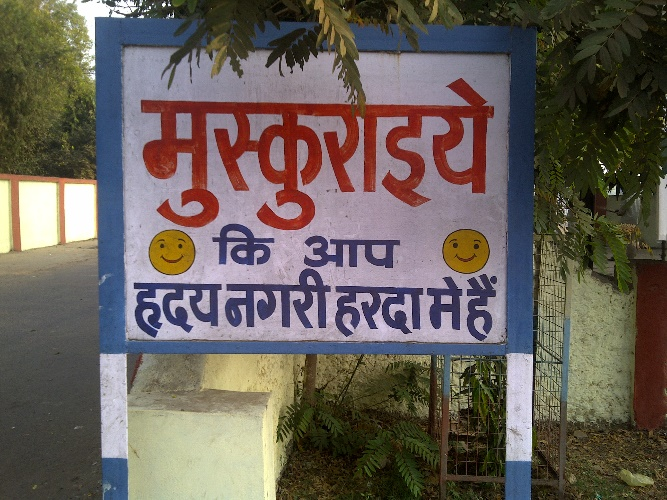
\includegraphics[width=2.6in]{harda}
	  	% \caption{Harda College}
	  	\label{fig:sub1}
	\end{subfigure}%
	\begin{subfigure}{.5\textwidth}
	  	\centering
	  	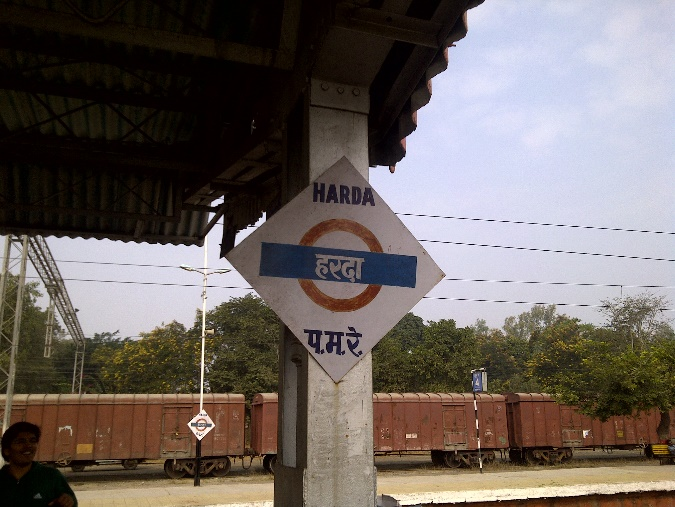
\includegraphics[width=2.6in]{railwayharda}
	  	% \caption{Active participants of EDP}
	  	\label{fig:sub2}
	\end{subfigure}
	\caption{Harda, Madhya Pradesh}
	\label{figstart}
\end{figure}


%%% Local Variables: 
%%% mode: latex
%%% TeX-master: "../thesis"
%%% End: 
